\documentclass{article}
\usepackage{graphicx}
\usepackage{subfiles}
\usepackage{subfigure}
\usepackage{color}
\graphicspath{{pics/}}

\title{Traitment numérique du signal \\ \vspace{5mm} Rapport sur le problème 2 \\ \vspace{3mm} Groupe G10C et } 
\author{MANGIN Rémi \\
LE MONNIER Romain \\
TEOFILOVIC Kristina \\
TON Sophie \\
RISY Théo \\
YANG Chen}   
\date{\today}  
\begin{document}

\maketitle

\newpage
\tableofcontents
\newpage

\textbf{Problème II :} \  \\
Proposer un algorithme qui permet de détecter, de caractériser une note de musique jouée par un instrument (violon, flûte, piano) et de déterminer sa hauteur. \\
Cet algorithme devra produire les sorties suivantes : \\
\begin{itemize}
    \item $t_d, t_f$: instants de début et de fin de note
    \item $P_dBm$: la puissance moyenne du signal en dBm
    \item $f_0$: la fréquence fondamentale et le nom et l'octave de la note jouée
    \item $f_h$: la fréquence haute telle que [0,$f_h$] contient 99.99\% de la puissance
    \item $n_h$: le nombre d'harmoniques dans cette bande de fréquences
    \item Toutes autres caractéristiques qui vous paraît pertinente pour classifier les notes par instrument de musique.
    On reprendra la méthode de détection d'un son utile du PBI et on justifiera les paramètres retenus.
\end{itemize}

\textbf{Problème IV :} \ \\
On souhaite détecter les signaux environnementaux qui comprennent des composantes spectrales très aiguës et pénibles pour l'oreille humaine. Ces signaux sont définis ainsi : 20\% de leur puissance est comprise dans les fréquences supérieures à 2 kHz, avec une puissance sonore totale supérieure à 110 dB SLP. \\
Concevoir un système de détection de ces signaux pénibles fondé sur filtrage
numérique. On prendra un micro de sensibilité égale à -67 dBV et de gain égal à 16 dB. Discuter les critères énoncés.

  
\newpage
\textcolor{blue}{\section{Introduction}}
Nous proposons une approche novatrice visant à élaborer un algorithme de détection et de caractérisation des notes de musique jouées par divers instruments tels que le violon, la flûte et le piano, tout en déterminant précisément leur hauteur. Notre algorithme est conçu pour générer des sorties exhaustives, incluant les instants de début et de fin de chaque note ($t_d$,$t_f$), la puissance moyenne du signal en dBm ($P_{dBm}$), la fréquence fondamentale ($f_0$) accompagnée du nom et de l’octave de la note jouée, la fréquence haute $f_h$ définie par [0, $f_h$] englobant 99.99\% de la puissance, le nombre d’harmoniques dans cette bande de fréquences ($n_h$), ainsi que toute autre caractéristique jugée pertinente pour classifier les notes selon l'instrument de musique. Nous adopterons la méthode de détection d’un son utile du PBI (Produit de l'analyse du Bruit Instantané) pour élaborer notre algorithme, en nous appuyant sur une approche en trois étapes. Cette méthodologie implique la détection du signal sonore, la synchronisation du récepteur par la détection de l'en-tête, et enfin, le décodage des informations pertinentes pour caractériser chaque note. 

\textcolor{blue}{\section{Méthode}}
\begin{figure}[htb]
    \centering
    \center{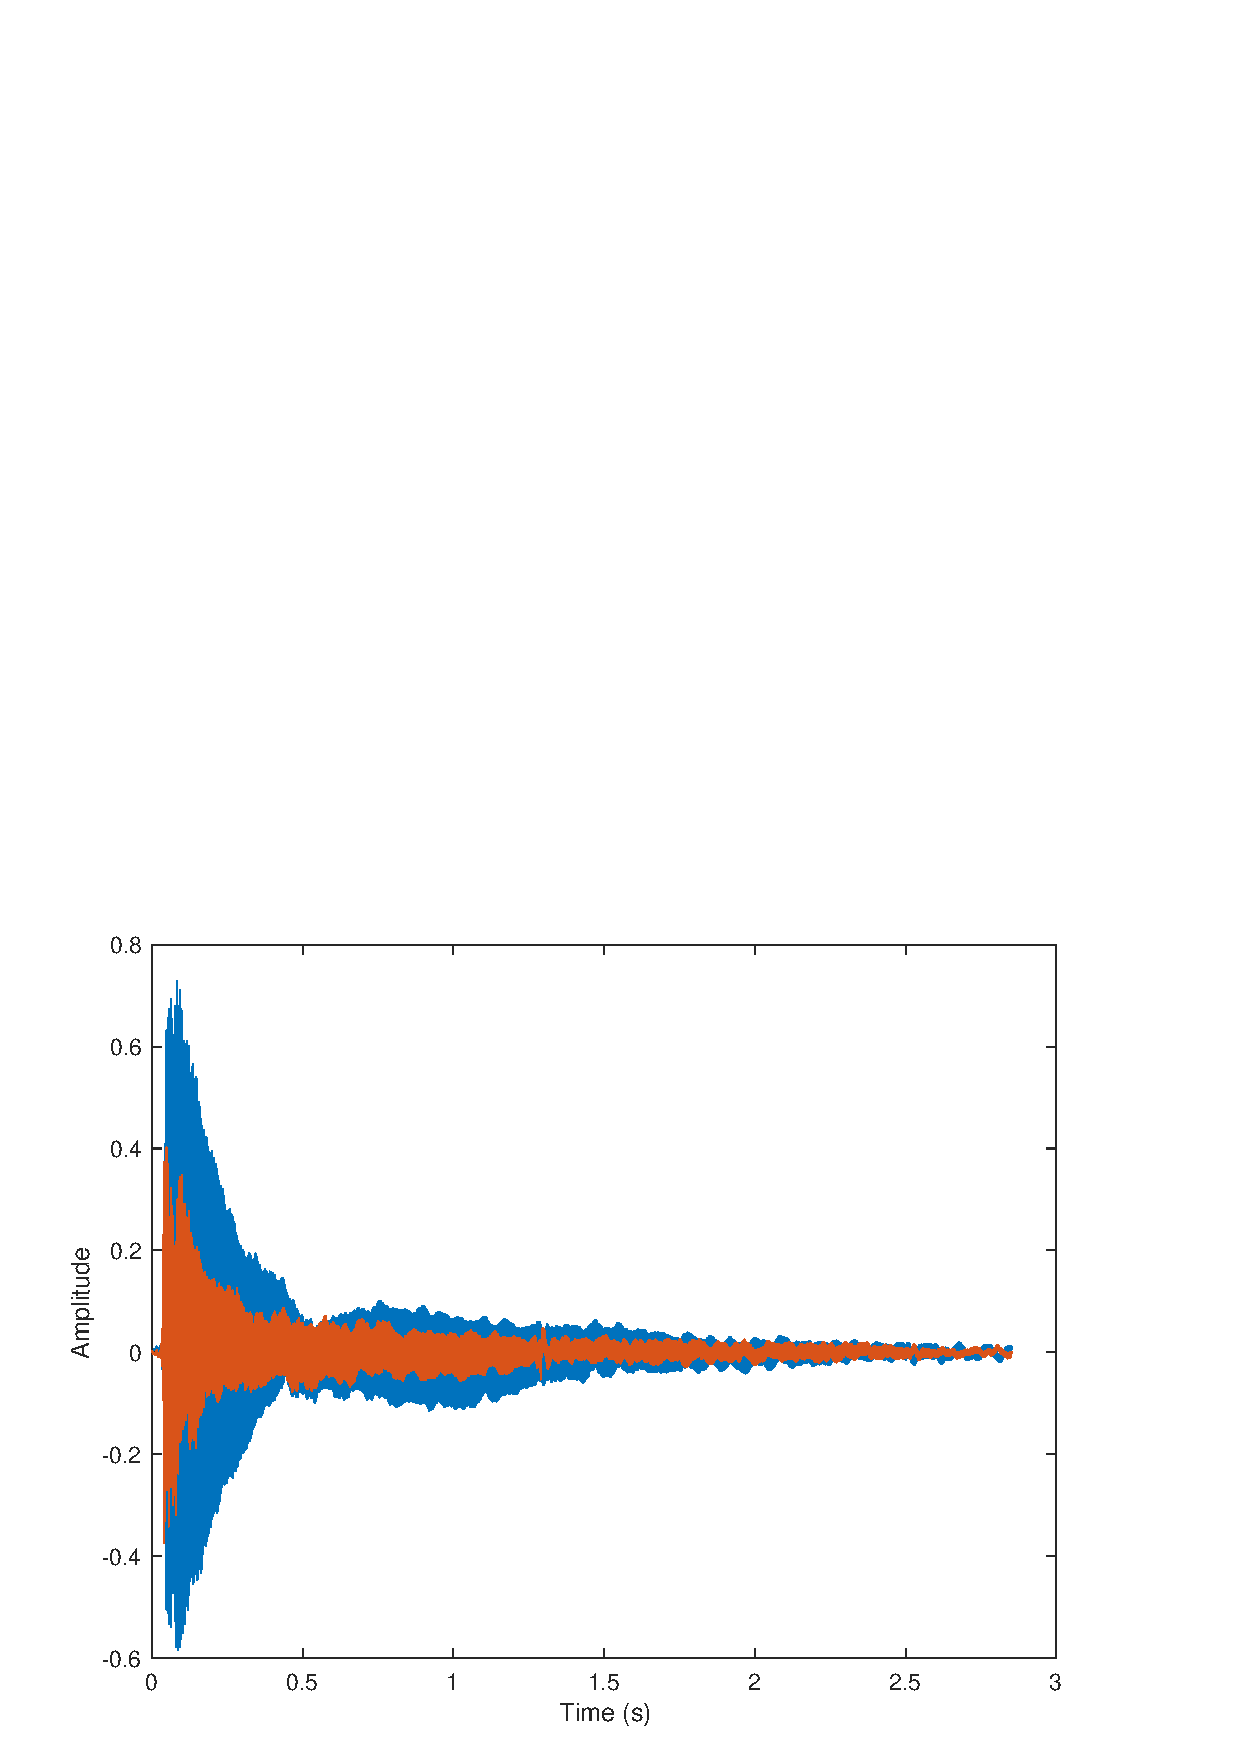
\includegraphics[width = 0.7\textwidth]{Semaine3/Problems2/rapport/pics/signal_before_mean.jpg}}
\end{figure}

\textcolor{blue}{\subsection{Acquisition et Pré-traitement du Signal}}
Dans cette première étape, nous chargeons une série de fichiers audio correspondant à différentes notes jouées par des instruments tels que le violon, la flûte et le piano. Ces fichiers audio sont ensuite convertis en signaux mono pour simplifier l'analyse. Pour chaque signal, nous calculons la puissance du signal en utilisant une fenêtre glissante de taille fixe. La puissance ainsi obtenue est ensuite convertie en décibels (dBm). Ensuite, nous effectuons une transformée de Fourier rapide sur le signal pour obtenir un spectre.Ce processus est essentiel pour préparer le signal en vue de l'analyse ultérieure. 
\textcolor{blue}{\subsection{Détection des Notes}}
La détection se fait en trouvant les points où la puissance du signal dépasse un seuil défini (1\% de la puissance maximale). Les indices correspondants sont ensuite convertis en temps, fournissant ainsi les instants de début et de fin de chaque note. Les notes d'une durée inférieure à une seconde sont éliminées pour garantir la qualité des données. 
Fig.\ref{fig:Note_Detection} est le signal avec les notes détectées(partie rouge).
\newpage
\begin{figure}[htb]
    \centering
    \includegraphics[width=0.8\textwidth]{signal_with_note_detected.png}
    \caption{Exemple signal avec les notes détectées}
    \label{fig:Note_Detection}
\end{figure}
\textcolor{blue}{\subsection{Détermination de la Fréquence Fondamentale}}
Le décodage des caractéristiques de chaque note s'effectue en calculant la puissance moyenne, la fréquence fondamentale ($f_0$), la fréquence de la plus haute harmonique ($f_h$), et le nombre d'harmoniques dans la bande de fréquences.La détection précise de la fréquence fondamentale ($f_0$) est essentielle dans l'analyse des signaux sonores, notamment pour l'étude des notes musicales. Ces informations sont extraites à partir du signal audio, utilisant diverses fonctions telles que le calcul de la moyenne de puissance, la fréquence fondamentale par auto-corrélation, et le comptage des harmoniques. Les résultats sont affichés pour chaque note, fournissant une caractérisation détaillée des éléments musicaux contenus chaque fichier audio ainsi que la note et l'octave associée à la fréquence. 

L'ensemble de ces étapes contribue à élaborer un algorithme complet de détection et de caractérisation des notes de musique, avec une option facultative pour estimer la direction de la source sonore sur des signaux acquis par deux micros différents. 

Dans notre étude, nous avons appliqué deux méthodes distinctes pour calculer cette fréquence fondamentale, puis nous les avons comparées afin de vérifier leur exactitude.

La première méthode s'appuie sur la détection de la fréquence qui présente la densité de puissance la plus élevée après avoir effectué une transformation de Fourier rapide (FFT). Cette approche est basée sur l'hypothèse que, dans la majorité des cas, la fréquence fondamentale correspond à la fréquence la plus basse ayant la plus grande densité de puissance.
\begin{equation}
    f_0 = \arg\max_f(\frac{2}{N}|FFT(signal)|)
\end{equation}

Quant à la seconde méthode, nous utilisons le principe de l'auto-corrélation dans le domaine temporel. Cette technique permet de détecter les répétitions périodiques au sein du signal, ce qui facilite l'identification de la fréquence fondamentale, même en présence de harmoniques complexes ou de bruit.
\begin{equation}
    f_0 = \frac{f_s}{Lag_{peak}}
\end{equation}
Où: 
\begin{itemize}
    \item $f_0$ est la fréquence fondamentale  
    \item $f_s$ est la fréquence d'échantillonnage 
    \item $Lag_{peak}$ est le temps de retard correspondant au premier pic significatif de la fonction d'auto-corrélation.
\end{itemize}

Ces méthodes contribuent à élaborer un algorithme complet de détection et de caractérisation des notes de musique. En combinant et en comparant les résultats obtenus par ces deux méthodes, nous pouvons augmenter la fiabilité de notre analyse et assurer une détection plus précise de la fréquence fondamentale, ce qui est crucial pour une compréhension approfondie des propriétés acoustiques des notes analysées.

\textcolor{blue}{\subsection{Analyse des Harmoniques}}
Dans l'analyse des signaux audio, la détection précise des harmoniques est essentielle pour comprendre les caractéristiques spectrales du signal.

Notre recherche utilise une méthode basée sur la transformée de Fourier rapide (FFT) pour identifier les composantes harmoniques d'un signal. Ce processus consiste à calculer la FFT du signal et à en extraire les points de fréquence qui répondent à des conditions spécifiques et qui représentent les composantes harmoniques.

Tout d'abord, nous effectuons une FFT sur le signal original pour obtenir son spectre, et nous ne considérons que la partie positive de la fréquence. Dans le spectre, nous identifions d'abord le point de fréquence ayant le puissance la plus élevée (\(P_{max}\)), et à partir de là, une seuil relatif est fixé (typiquement 40dB en dessous du point de puissance maximale). Tous les points de fréquence supérieurs à ce seuil sont initialement reconnus comme des harmoniques possibles.

Ensuite, pour chaque multiple entier de la fréquence fondamentale (\(n \times f_0 \), où n est un nombre naturel), nous recherchons les points du spectre qui sont les plus proches de ces fréquences. Si les fréquences de ces points ne dépassent pas un seuil de fréquence maximale fixé (\(f_{max}\)) avec une puissance d'au moins 10\% de la puissance maximale, ces points de fréquence sont identifiés comme des harmoniques. De cette manière, nous pouvons extraire efficacement les composante harmoniques du signal.
\begin{equation}
    Harmonics = \{f_n | f_n = n \times f_0, n \in \mathbb{N}, f_n \leq f_{max}, P(f_n) \geq 0.1 \times P_{max} \}
\end{equation}
où:
\begin{itemize}
    \item \(f_n\) est la fréquence de la nième harmonique
    \item \(f_0\) est la fréquence fondamentale
    \item \(P(f_n)\) est la densité spectrale de puissance à la fréquence \(f_n\)
    \item \(P_{max}\) est la maxime dans le spectrale de fréquence 
    \item \(f_{max}\) est le seuil de fréquence le plus élevé pour la détection des harmoniques
\end{itemize}

\newpage
\textcolor{blue}{\section{Résultats Expérimentaux}}
\begin{document}
ici est resultats
\end{document}
\newpage
\textcolor{blue}{\section{Conclusion}}
\begin{document}
ici est conclusion
\end{document}
\end{document}